%-----------------------------------------------------------------------------------------------------------------------------------------------%
%	The MIT License (MIT)
%
%	Copyright (c) 2016 Jan Küster
%
%	Permission is hereby granted, free of charge, to any person obtaining a copy
%	of this software and associated documentation files (the "Software"), to deal
%	in the Software without restriction, including without limitation the rights
%	to use, copy, modify, merge, publish, distribute, sublicense, and/or sell
%	copies of the Software, and to permit persons to whom the Software is
%	furnished to do so, subject to the following conditions:
%	
%	THE SOFTWARE IS PROVIDED "AS IS", WITHOUT WARRANTY OF ANY KIND, EXPRESS OR
%	IMPLIED, INCLUDING BUT NOT LIMITED TO THE WARRANTIES OF MERCHANTABILITY,
%	FITNESS FOR A PARTICULAR PURPOSE AND NONINFRINGEMENT. IN NO EVENT SHALL THE
%	AUTHORS OR COPYRIGHT HOLDERS BE LIABLE FOR ANY CLAIM, DAMAGES OR OTHER
%	LIABILITY, WHETHER IN AN ACTION OF CONTRACT, TORT OR OTHERWISE, ARISING FROM,
%	OUT OF OR IN CONNECTION WITH THE SOFTWARE OR THE USE OR OTHER DEALINGS IN
%	THE SOFTWARE.
%
%	RESOURCES USED:
%	http://tex.stackexchange.com/questions/5718/package-for-pie-charts
%	http://tex.stackexchange.com/questions/183087/draw-colored-world-us-map-in-latex#183138
%	http://www.texample.net/tikz/examples/simple-flow-chart/
%	http://vizualize.me/#
%-----------------------------------------------------------------------------------------------------------------------------------------------%


%============================================================================%
%
%	DOCUMENT DEFINITION
%
%============================================================================%

%we use article class because we want to fully customize the page
\documentclass[10pt,A4]{article}	


%----------------------------------------------------------------------------------------
%	ENCODING
%----------------------------------------------------------------------------------------

%we use utf8 since we want to build from any machine
\usepackage[utf8]{inputenc}		

%----------------------------------------------------------------------------------------
%	LOGIC
%----------------------------------------------------------------------------------------

% provides \isempty test
\usepackage{xifthen}
\usepackage{calc}

%----------------------------------------------------------------------------------------
%	FONT
%----------------------------------------------------------------------------------------

% some tex-live fonts - choose your own

%\usepackage[defaultsans]{droidsans}
%\usepackage[default]{comfortaa}
%\usepackage{cmbright}
\usepackage[default]{raleway}
%\usepackage{fetamont}
%\usepackage[default]{gillius}
%\usepackage[light,math]{iwona}
%\usepackage[thin]{roboto} 

% set font default
\renewcommand*\familydefault{\sfdefault} 	
\usepackage[T1]{fontenc}

% more font size definitions
\usepackage{moresize}		


%----------------------------------------------------------------------------------------
%	PAGE LAYOUT  DEFINITIONS
%----------------------------------------------------------------------------------------

%debug page outer frames
%\usepackage{showframe}			


%define page styles using geometry
\usepackage[a4paper]{geometry}		

% for example, change the margins to 2 inches all round
\geometry{top=0.75cm, bottom=-.6cm, left=1cm, right=1cm} 	


%use customized header
\usepackage{fancyhdr}				
\pagestyle{fancy}

%less space between header and content
\setlength{\headheight}{-5pt}		


%customize entries left, center and right
\lhead{}
\rhead{}

\setlength{\parindent}{0mm}	%indentation is zero

%----------------------------------------------------------------------------------------
%	TABLE /ARRAY DEFINITIONS
%---------------------------------------------------------------------------------------- 

\usepackage{multicol}			
\usepackage{multirow}

\usepackage{array}	%extended aligning of tabular cells

\newcolumntype{x}[1]{%
>{\raggedleft\hspace{0pt}}p{#1}}%


%----------------------------------------------------------------------------------------
%	GRAPHICS DEFINITIONS
%---------------------------------------------------------------------------------------- 

\usepackage{graphicx}	%for header image
\usepackage{wrapfig}	%for floating figures
\usepackage{float}
%\floatstyle{boxed} 
%\restylefloat{figure}

		
\usepackage{tikz}	%for drawing graphics
\usetikzlibrary{shapes, backgrounds}

%http://tex.stackexchange.com/questions/7219/how-to-vertically-center-two-images-next-to-each-other
\newcommand{\vcenteredinclude}[1]{\begingroup
\setbox0=\hbox{\includegraphics{#1}}%
\parbox{\wd0}{\box0}\endgroup}

%http://tex.stackexchange.com/questions/7219/how-to-vertically-center-two-images-next-to-each-other
\newcommand*{\vcenteredhbox}[1]{\begingroup
\setbox0=\hbox{#1}\parbox{\wd0}{\box0}\endgroup}


\newcommand{\icons}{Font-Awesome-SVG-PNG/white/png/64/}	%path to your icon lib
\newcommand{\icon}[2]{\includegraphics[height=#2]{\icons#1}}	%icon shortcut
\newcommand{\icontext}[3]{ 						%icon with text shortcut
	\vcenteredhbox{\icon{#1}{#2}} \vcenteredhbox{#3}
}

%----------------------------------------------------------------------------------------
%	Color DEFINITIONS
%---------------------------------------------------------------------------------------- 

\usepackage{color}

%accent color
\definecolor{sectcol}{RGB}{255,150,0}

\definecolor{secondcol}{RGB}{50,50,200}

%dark background color
\definecolor{bgcol}{RGB}{100,100,100}

%light background / accent color
\definecolor{softcol}{RGB}{225,225,225}

%background col for whole page
\pagecolor{bgcol}

%============================================================================%
%
%
%	DEFINITIONS
%
%
%============================================================================%

%----------------------------------------------------------------------------------------
% 	HEADER
%----------------------------------------------------------------------------------------

% remove top header line
\renewcommand{\headrulewidth}{0pt} 

%remove botttom header line
\renewcommand{\footrulewidth}{0pt}	  	

%remove pagenum
\renewcommand{\thepage}{}	

%remove section num		
\renewcommand{\thesection}{}			

\chead{}

%----------------------------------------------------------------------------------------
% 	ARROW GRAPHICS in Tikz
%----------------------------------------------------------------------------------------

% a six pointed arrow poiting to the left
\newcommand{\tzlarrow}{(0,0) -- (0.2,0) -- (0.3,0.2) -- (0.2,0.4) -- (0,0.4) -- (0.1,0.2) -- cycle;}	

% a six pointed arrow poiting to the right
\newcommand{\tzrarrow}{ (0,0.2) -- (0.1,0) -- (0.3,0) -- (0.2,0.2) -- (0.3,0.4) -- (0.1,0.4) -- cycle;}


% include the left arrow into a tikz picture
% param1: fill color
%
\newcommand{\larrow}[1]
{\begin{tikzpicture}[scale=0.58]
	 \filldraw[fill=#1!100,draw=#1!100!black]  \tzlarrow
 \end{tikzpicture}
}

% include the right arrow into a tikz picture
% param1: fill color
%
\newcommand{\rarrow}[1]
{\begin{tikzpicture}[scale=0.58]
	\filldraw[fill=#1!100,draw=#1!100!black] \tzrarrow
 \end{tikzpicture}
}


% draw a slice for a chart
% param 1:
% param 2:
% param 3:
% param 4:
% param 5:
% param 6:
\newcommand{\slice}[6] {
 	\pgfmathparse{0.5*#1+0.5*#2}
  	\let\midangle\pgfmathresult
	% slice
  	\filldraw[fill=#5!100,draw=bgcol!100, line width=2pt,  inner sep=15pt ] (0,0) -- (#1:#6) arc (#1:#2:#6) -- cycle;

%	\draw[draw=white]
  	% outer label
  	\node[label=\midangle:\textcolor{white}{#4}] at (\midangle:#6) {};
}

%counters for chart loop
\newcounter{a}
\newcounter{b}
\newcounter{c}

% draws a pie chart by a list of input values
% param 1: the value list ->example: 20/type A, 4/type B, 11/type C, 49/type D, 16/other
% param 2: scaling factor (no font scaling)
% param 3: circle size, use 90, 180, 270 or 360
% param 4: caption
\newcommand{\chart}[4]{
	%reset counters
	\setcounter{a}{0}
	\setcounter{b}{0}
	\setcounter{c}{50}
	\begin{tikzpicture}[scale=3]
	\foreach \p/\t in {#1} {
		\setcounter{a}{\value{b}}
	    	\addtocounter{b}{\p}
		\addtocounter{c}{35}
		\definecolor{currentcolor}{RGB}{220,\thec, 0}
	    	\slice{\thea/100*#3}{\theb/100*#3}{\p\%}{\t}{currentcolor}{#2}
	}
	\end{tikzpicture}
}

\newcommand{\bubble}[5]{
	\definecolor{tmpcol}{RGB}{50,50,#5}
	% slice
  	\filldraw[fill=tmpcol!100,draw=none] (#1,0.5) circle (#3);

  	% outer label
  	\node[label=\textcolor{white}{#4}] at (#1,0.7) {};
}

\newcommand{\bubbles}[2]{
	%reset counters
	\setcounter{a}{0}
	\setcounter{c}{150}
	\begin{tikzpicture}[scale=3]
	\foreach \p/\t in {#1} {
	    	\addtocounter{a}{1}
	    	\bubble{\thea/2}{\theb}{\p/25}{\t}{1\p0}
	}
	\end{tikzpicture}
}

\newcommand{\squares}[2]{
	%reset counters
	\setcounter{a}{0}
	\setcounter{b}{0}
	\setcounter{c}{50}
	\begin{tikzpicture}[scale=3]
	\foreach \p/\t in {#1} {
		\setcounter{a}{\value{b}}
	    	\addtocounter{b}{\p}
		\addtocounter{c}{35}
		\definecolor{currentcolor}{RGB}{50,50, 1\p}
	    	\square{\thea/100*#2}{\theb/100*#2}{\p\%}{\t}{currentcolor}
	}
	\end{tikzpicture}
}

\newcommand{\square}[5] {
 	\pgfmathparse{#1+0.5*(#2-#1)-0.14}
  	\let\midangle\pgfmathresult
	% slice
  	\filldraw[fill=#5!100,draw=bgcol!100, line width=3pt] (0,#1) -- (2,#1) -- (2,#2) -- (0,#2) -- cycle;
  	% outer label
  	\node[label=\textcolor{white}{#4}] at (1,\midangle) {};
}
%----------------------------------------------------------------------------------------
%	social info
%----------------------------------------------------------------------------------------



%----------------------------------------------------------------------------------------
%	custom sections
%----------------------------------------------------------------------------------------

% create a coloured box with arrow and title as cv section headline
% param 1: section title
%
\newcommand{\cvsection}[1] {
	\larrow{bgcol} \textcolor{white}{\textbf{#1}}  \rarrow{bgcol}
}

\newcommand{\cvsect}[2]{
	\colorbox{gray}{ \makebox[0.75\linewidth][c]{\cvsection{#1}}}
}

%create a coloured arrow with title as cv meta section section
% param 1: meta section title
%
\newcommand{\metasection}[2] {
	\begin{tabular*}{1\textwidth}{ l l }
		#1&#2\\[12pt]
	\end{tabular*}
}

%----------------------------------------------------------------------------------------
%	 CV EVENT
%----------------------------------------------------------------------------------------
\newcounter{expcounter}
\newcounter{educounter}
\newcounter{yearcount}
% creates a vertical cv timeline
% param 1: start year
% param 2: end year
% param 3: overall width
%param 4: overall height
\newenvironment{cvtimeline}[4]{
	% creates a stretched box as cv entry headline followed by two paragraphs about 
	% the work you did
	% param 1:	event start month/year
	% param 2:	event end month/year
	% param 3:  event name
	% param 4:	institution (where did you work / study)
	% param 5:	what was your position
	% param 6:	some words about your contributions
	%
	\newcommand{\cvexperience}[6] {
		
		\foreach \monthf/\yearf in {##1} {
			\foreach \montht/\yeart in {##2} {
				\definecolor{expcol}{RGB}{50,50,\theexpcounter}
				\pgfmathparse{#3/\fullrange*((\yearf-#1)+(\monthf/12))}
  				\let\startexp\pgfmathresult
				\pgfmathparse{#3/\fullrange*((\yeart-#1)+(\montht/12))}
  				\let\endexp\pgfmathresult
				\pgfmathparse{1/(\endexp-\startexp+1.5)}
  				\let\lenexp\pgfmathresult
				\pgfmathparse{0.5*\endexp+0.5*\startexp}
  				\let\midexp\pgfmathresult

				\draw[fill=expcol, opacity=0.75] (\startexp,-0.1) -- (\startexp,-0.6-\lenexp) -- (\endexp,-0.6-\lenexp) -- (\endexp,-0.1) --cycle;
				\draw[draw=black](\midexp,-0.6-\lenexp) -- ((\midexp,-1.5-\lenexp);
				\node[label=\textcolor{black}{##3}] at (\midexp,-2-\lenexp) {}; %start year
				\addtocounter{expcounter}{50}
			}
		}
	}
	\newcommand{\cveducation}[6] {
		\foreach \monthf/\yearf in {##1} {
			\foreach \montht/\yeart in {##2} {
				\definecolor{expcol}{RGB}{250,\theeducounter,0}
				\pgfmathparse{#3/\fullrange*((\yearf-#1)+(\monthf/12))}
  				\let\startexp\pgfmathresult
				\pgfmathparse{#3/\fullrange*((\yeart-#1)+(\montht/12))}
  				\let\endexp\pgfmathresult
				\pgfmathparse{1/(\endexp-\startexp+1.5)}
  				\let\lenexp\pgfmathresult
				\pgfmathparse{0.5*\endexp+0.5*\startexp}
  				\let\midexp\pgfmathresult

				\draw[fill=expcol, opacity=0.75] (\startexp,0.1) -- (\startexp,0.6+\lenexp) -- (\endexp,0.6+\lenexp) -- (\endexp,0.1) --cycle;
				\draw[draw=black](\midexp,0.6+\lenexp) -- ((\midexp,1+\lenexp);
				\node[label=\textcolor{black}{##3}] at (\midexp,1.1+\lenexp) {}; %start year
				\addtocounter{educounter}{50}
			}
		}
	}
	\begin{tikzpicture}
 	\pgfmathparse{(#2-#1)}
  	\let\fullrange\pgfmathresult
	\draw[draw=white,line width=1pt] (0,0) -- (#3,0) ;	%line

	%for each year put a horizontal line in place
	\setcounter{yearcount}{1}
	\setcounter{expcounter}{50}
	\whiledo{\value{yearcount} < \fullrange}{
		\draw[draw=white] (#3/\fullrange*\value{yearcount},-0.15) -- (#3/\fullrange*\value{yearcount},0.15);
		\stepcounter{yearcount}
	}
	\node[label=\textcolor{white}{#1}] at (-0.75,0) {}; %start year
	\node[label=\textcolor{white}{#2}] at (#3+0.75,0) {}; %end year
	
}%end begin part of newenv
{\end{tikzpicture}}

% creates a stretched box as 
\newcommand{\cveventmeta}[2] {
	\mbox{\mystrut \hspace{87pt}\textit{#1}}\\
	#2
}

%----------------------------------------------------------------------------------------
% CUSTOM STRUT FOR EMPTY BOXES
%----------------------------------------- -----------------------------------------------
\newcommand{\mystrut}{\rule[-.3\baselineskip]{0pt}{\baselineskip}}

%----------------------------------------------------------------------------------------
% CUSTOM LOREM IPSUM
%----------------------------------------------------------------------------------------
\newcommand{\lorem}{Lorem ipsum dolor sit amet, consectetur adipiscing elit. Donec a diam lectus.}


%============================================================================%
%
%
%
%	DOCUMENT CONTENT
%
%
%
%============================================================================%
\begin{document}


%use our custom fancy header definitions
\pagestyle{fancy}	


%---------------------------------------------------------------------------------------
%	TITLE HEADLINE
%----------------------------------------------------------------------------------------
\mystrut
\vspace{-12pt}
\begin{center}
\HUGE{\textcolor{white}{\textsc{Jan Küster}} }\\[-30pt]
\textcolor{sectcol}{\hrule}
\vspace{5pt}
\Large{\textcolor{white}{\textsc{Software Engineer and Consultant}}}\\
\end{center}

\normalfont


%---------------------------------------------------------------------------------------
%	QR CODE (optional)
%----------------------------------------------------------------------------------------
%\vspace{-136pt}
%\hspace{0.75\linewidth}
%
\includegraphics[width=103pt]{qrcode}
%\normalsize
%\vspace{88pt}



%---------------------------------------------------------------------------------------
%	META SECTION
%----------------------------------------------------------------------------------------
\vspace{16pt}

\begin{minipage}{0.49\textwidth}
	\begin{center}
		\cvsect{Profile}{0.49}\\[16pt]
	\end{center}

\begin{tabular*}{1\textwidth}{ c c }
	\parbox[c]{0.375\linewidth}{
	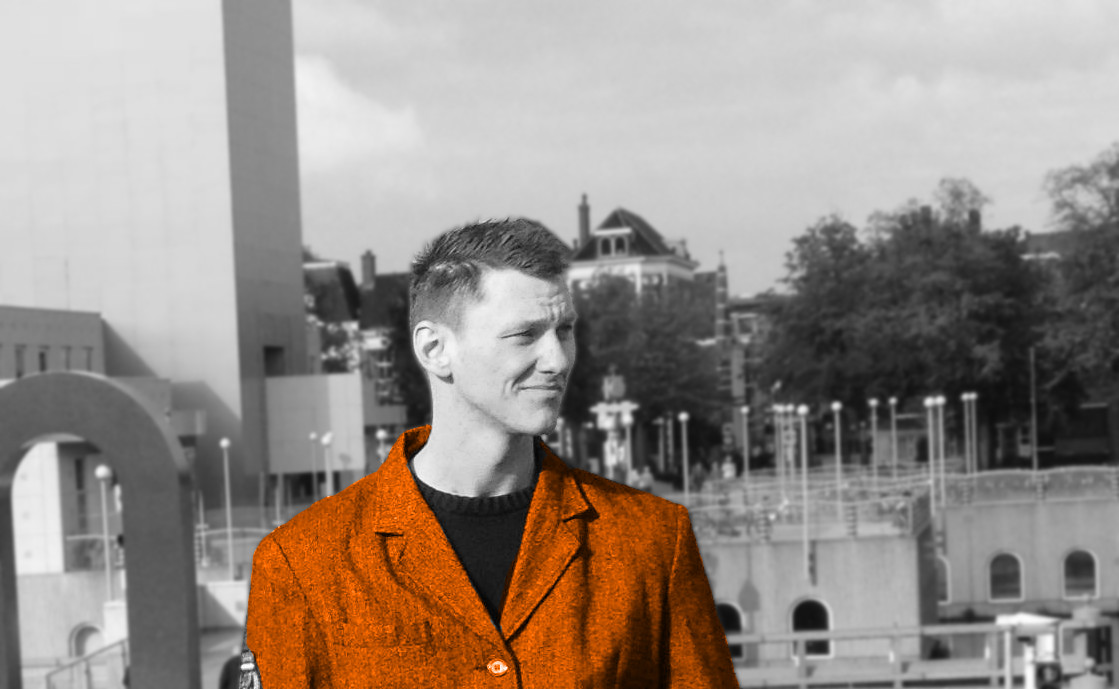
\includegraphics[trim= 320 130 460 210,clip,width=\linewidth]{myfoto.jpg}}&
	\parbox{0.55\textwidth}{
	\icontext{map-marker}{22pt}{Bremen, Germany}\\
	\icontext{mobile-phone}{22pt}{+49 176 313 877 34}\\
	\icontext{send}{22pt}{info@jankuester.com}\\
	\icontext{mouse-pointer}{22pt}{www.jankuester.com}\\
	\icontext{github}{22pt}{github.com/jankapunkt}\\
	\icontext{twitter}{22pt}{@Kuester\_Jan}\\
	}
\end{tabular*}

\end{minipage}
\begin{minipage}{0.49\textwidth}
	\begin{center}
		\cvsect{Skills}{0.49}\\[16pt]
		\chart{9/Design, 25/Consulting, 25/Projects,41/Development}{0.65}{360}{nothing}\\[16pt]

	\end{center}
\end{minipage}

\vspace{16pt}

\begin{center}
	\cvsect{Experience and Education}{0.49}\\[16pt]

\end{center}

\begin{cvtimeline}{2009}{2017}{15.5}{\linewidth}
%---------------------------------------------------------------------------------------
%	EXPERIENCE
%----------------------------------------------------------------------------------------


\cvexperience{11/2014}{9/2016}{IT Consultant}{We4IT GmbH Bremen}{Realize projects in XPages and We4IT Aveedo, monitor project status, conduct reports}{Implement the frontend for a BPMN compatible engine within We4IT Aveedo}

\cvexperience{9/2013}{9/2013}{Poster Presentation}{DELFI Conference}{Co-published poster with paper on usability guidelines for tests with functional illiterates}{Presented results to conference audience at conference event}

\cvexperience{1/2012}{11/2014}{Scientific Employee}{Uni of Bremen}{Invented a flexible assessment framework, targeting industrial trainees}{Supervised software development lifecycle, Recruited team members}



\cvexperience{6/2010}{11/2011}{Student Assistant}{Uni Bremen}{Realized an online diagnosis platform for workforce literacy development (Flex)}{Modeled software design, implemented various prototypes, conducted usability tests}

\cvexperience{05/2016}{05/2016}{Startup Weekend}{Getoq Consulting}{Performed a two-day project simulation from management perspective}{Topics included customer contracts, change management, controlling, operational tasks}



%---------------------------------------------------------------------------------------
%	EDUCATION SECTION
%--------------------------------------------------------------------------------------

\cveducation{1/2009}{11/2011}{Bachelor Studies}{University of Bremen}{Master Thesis: Semi Automated Scoring in Technology Based Assessment}{Developed and evaluated an algorithm for semi automated scoring of spreadsheet data}


\cveducation{7/2015}{7/2015}{M.Sc. Graduation}{University of Bremen}{Master Thesis: Semi Automated Scoring in Technology Based Assessment}{Developed and evaluated an algorithm for semi automated scoring of spreadsheet data}

\cveducation{11/2011}{11/2011}{PM Seminar}{Getoq Consulting}{Performed a two-day project simulation from management perspective}{Topics included customer contracts, change management, controlling, operational tasks}

%\cvevent{2012 - 2013}{Master Project - PrIMA}{University of Bremen}{Co-Invented a touch table application for medical support, co-developed software (Java) }{Formed a scrum team, mainted project dev server (Debian), surveyed target audience}

%\textcolor{softcol}{\hrule}

\cveducation{11/2011}{7/2015}{Master Studies Digital Media}{University of Bremen}{Inter-cultural classes in English, covering special topics in computer science and design}{Professionalized in research methods, software development and e-assessment}

%\textcolor{softcol}{\hrule}

\cveducation{5/2009}{1/2010}{Semester Abroad}{University of Melbourne}{Mastered six months of study and trans-cultural experience in Melbourne, Australia}{Finished machine programming, information visualization, professional essay writing}
		\end{cvtimeline}\\

\begin{minipage}{0.49\textwidth}
	\begin{center}

		\cvsect{Technologies}{0.49}\\[16pt]
		\bubbles{6/js , 3/java , 3/Meteor , 2/React, 2/Notes}{\cvsection{Technologies}}\\[16pt]
		\bubbles{5/git, 5/eclipse, 2/excel, 2/LaTex}{\cvsection{Technologies}}\\[16pt]

		\cvsect{Activities}{0.49}\\[16pt]
		\squares{10/Game Development,40/Martial Arts,30/News,20/Music}{1.5}\\[6pt]
	\end{center}
\end{minipage}
\begin{minipage}{0.49\textwidth}
	\begin{center}
		\cvsect{Languages}{0.49}\\[12pt]
		German (native) English (Academic) Russian (Basic)\\[4pt]
		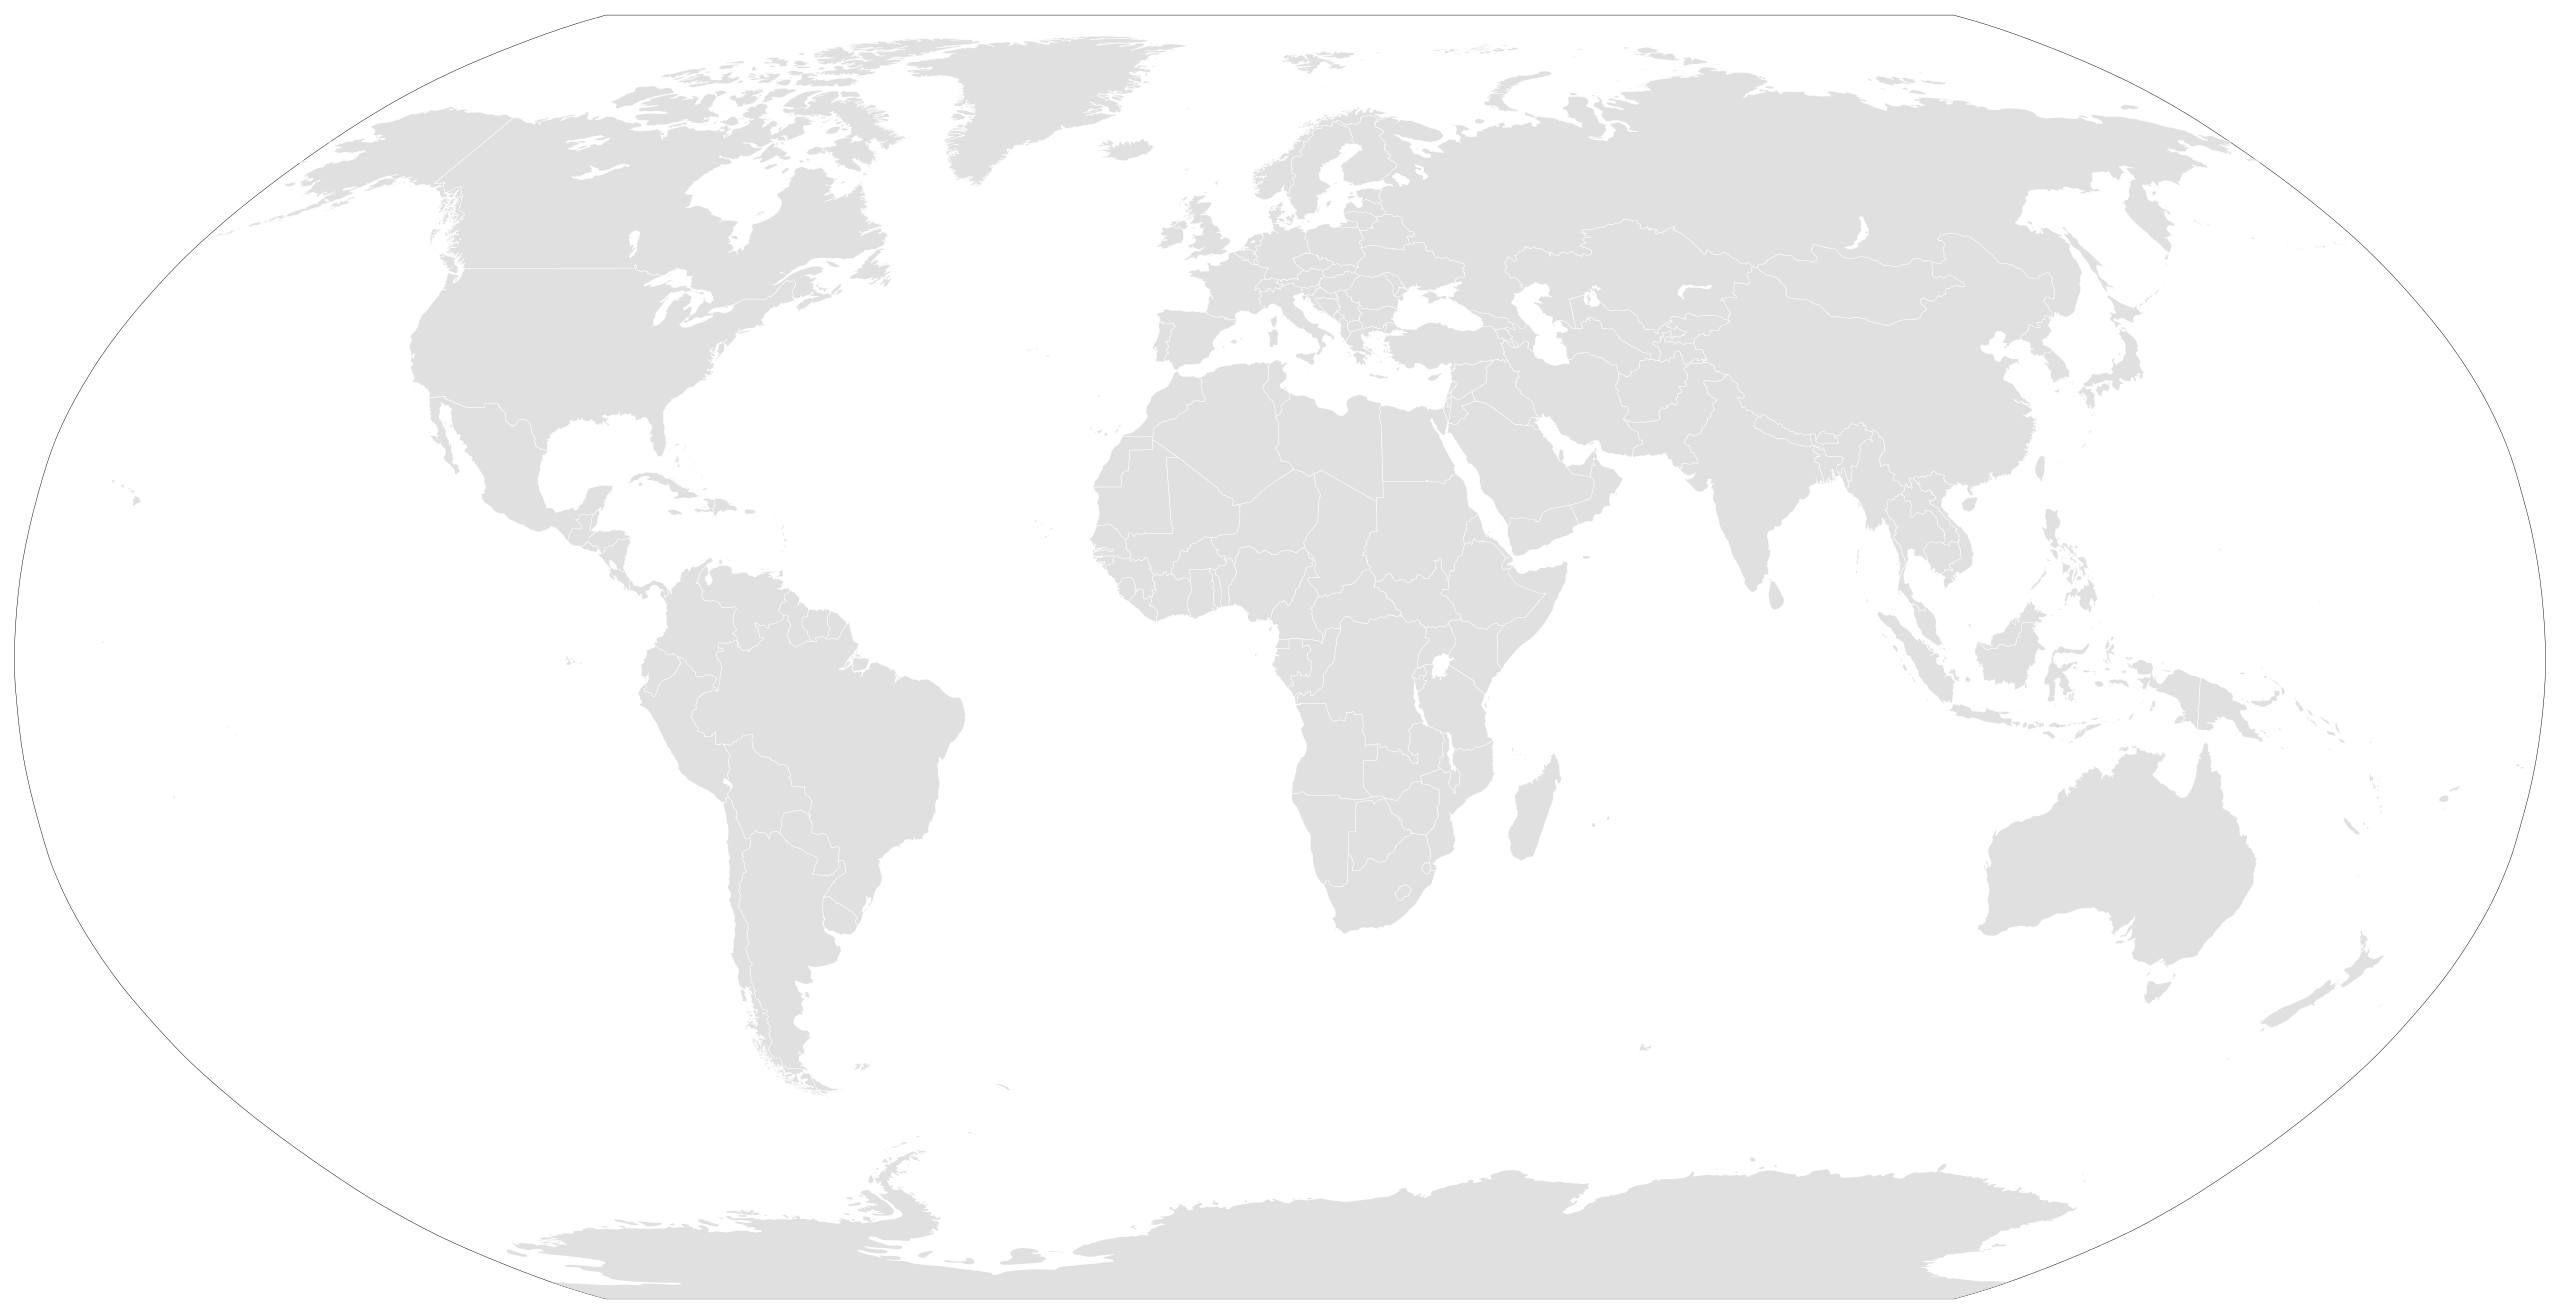
\includegraphics[width=1\linewidth]{world.png}\\[12pt]	 %trimming relative to image size!		


	\end{center}
\end{minipage}
%============================================================================%
%
%
%
%	DOCUMENT END
%
%
%
%============================================================================%
\end{document}
